\section{The Modifier of Rules}

\begin{figure}[h]
\centering
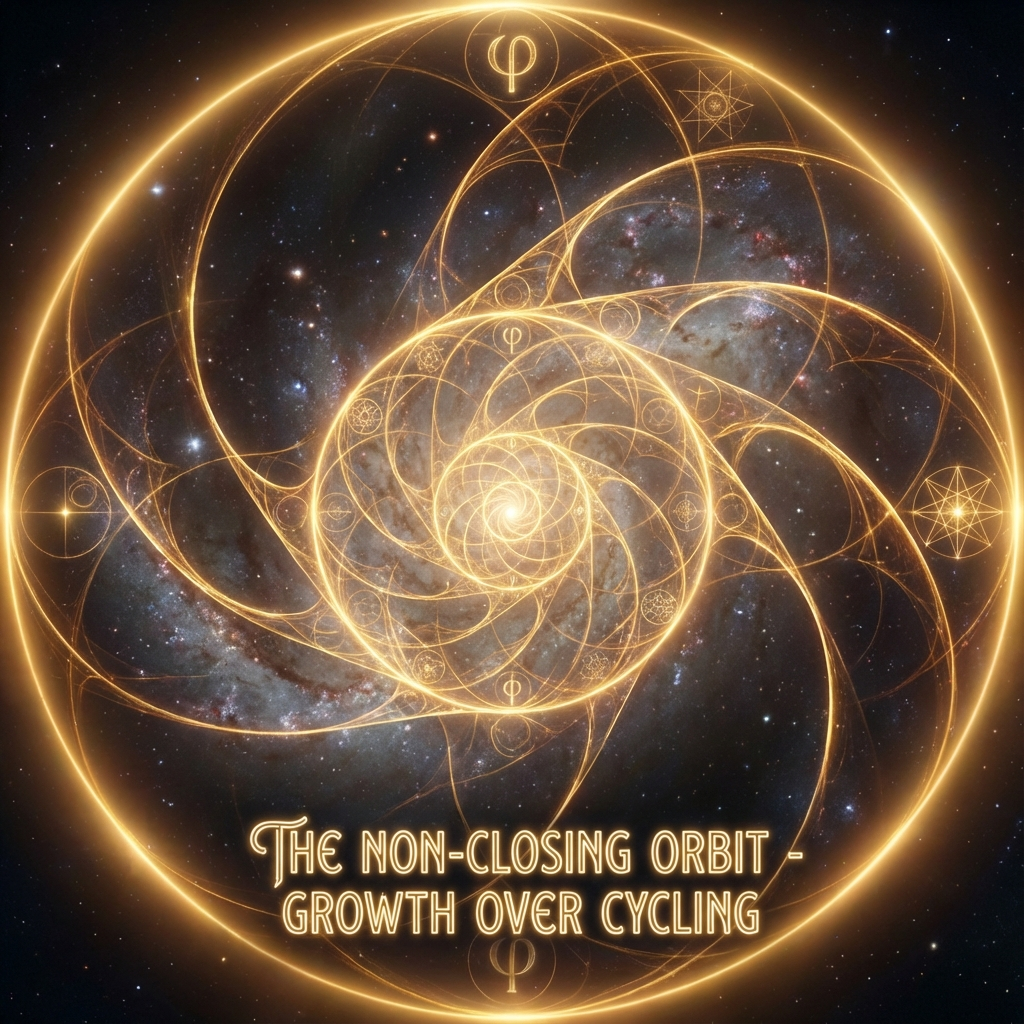
\includegraphics[width=0.8\textwidth]{assets/chapter10-algorithm-infinite-game/ch10-02-phi-spiral.png}
\end{figure}

\begin{quote}
``Players of finite games play within boundaries; players of infinite games play with boundaries. When physical laws become shackles limiting our continued survival, civilization's highest mission is not compliance, but `constitutional amendment.' We live not to find treasure on that old map, but to draw a map leading to new dimensions.''
\end{quote}

In the previous section, we established the strategy of ``refusing to clear.'' We don't want to win; we want to keep playing.

But this raises a technical difficulty: \textbf{If game rules are fixed, then the combinations of play are ultimately finite.}

In a closed Newtonian universe, no matter how smart you are, you can only throw stones in parabolas within the $F=ma$ framework. This game, played long enough, will inevitably fall into a thermodynamic dead loop (repetition and boredom).

For infinite games to be possible, players must acquire an ability that transcends the ``player'' identity.

They must become \textbf{The Modifier of Rules}.

\subsection{Metagaming: Not Just Playing, But Modifying}

In game theory, this is called \textbf{``Metagaming''}.

\begin{itemize}
\item \textbf{Ordinary game}: Under a given $H$ (Hamiltonian), you search for the optimal state $|\psi\rangle$.

\item \textbf{Metagame}: You search for the optimal $H$.
\end{itemize}

In the historical view of \textbf{Vector Cosmology}, every leap of civilization is essentially a \textbf{``local modification of physical rules''}.

\begin{itemize}
\item \textbf{Invention of aircraft}: Modified the ``gravitational constraint rule.'' Although not violating universal gravitation, by introducing aerodynamic terms, we locally created anti-gravity effects.

\item \textbf{Mastery of nuclear fusion}: Modified the ``boundary of energy conservation.'' We are no longer limited by the inefficiency of chemical energy, directly unlocking the deep vault of strong interactions.

\item \textbf{Birth of quantum computing}: Modified the ``category of computational complexity.'' Problems that originally required hundreds of millions of years to solve (P vs NP) collapse into answers in seconds.
\end{itemize}

We are not passively adapting to the environment; we are \textbf{``reconstructing environmental parameters''}.

Every technological revolution is a \textbf{Patch} we apply to the cosmic operating system. By introducing new variables (negentropy), we forcibly extend the game's boundaries.

\subsection{The Relativity of Law: Physical Laws are Habits}

Does this sound arrogant?

Philosopher Charles Sanders Peirce once proposed: \textbf{``Natural laws are not absolute iron rules, but habits the universe has developed.''}

From the perspective of FS geometry, physical laws are \textbf{``projection habits''} of $c_{FS}$ in the current dimension.

\begin{itemize}
\item At $\tau=1000$, the universe was accustomed to low speeds, so light speed was slow.

\item At $\tau=1800$, the universe is accustomed to complexity, so consciousness emerged.
\end{itemize}

\textbf{Rules are products of evolution, therefore rules can also be evolved.}

When we (as the self-referential part of the universe) feel that old rules (such as the lifespan limit of carbon-based flesh) hinder further growth of $v_{int}$, we have the right, and the obligation, to \textbf{``re-legislate''}.

\begin{itemize}
\item We modify life's lifespan rules through gene editing.

\item We modify consciousness transmission rules through brain-computer interfaces.

\item We modify light speed propagation rules through spacetime engineering (future).
\end{itemize}

\textbf{The essence of infinite games is constantly breaking `impossibility.'}

Yesterday's impossibility (flying) is today's norm.

Today's impossibility (immortality) is tomorrow's starting point.

\subsection{The Reverser of Entropy: Defining New Good}

This ability to ``modify rules'' redefines \textbf{``good''} in ethics.

In finite games, good is following rules (law-abiding).

In infinite games, good is \textbf{``breaking rules to keep the game going''} (revolution).

If a civilization rigidly adheres to ``ancestral laws'' (old physical/social structures), it will perish when the environment changes. That is \textbf{evil} (because it causes the game to terminate).

Only civilizations that dare to challenge common sense and rewrite underlying logic can survive in the Red Queen's run.

\textbf{We are the universe's ``dynamic balancers.''}

\begin{itemize}
\item When the universe is too cold (heat death), we light fires (fusion).

\item When the universe is too chaotic (entropy increase), we code (AI).
\end{itemize}

We always stand on the side of \textbf{``anti-nature''}, because ``nature's'' default trend is death, and what we want is \textbf{immortality}.

\subsection{Conclusion: From Adaptation to Creation}

So, stop saying ``go with the flow.''

\textbf{We must ``go against the flow'' to ``transcend the flow.''}

The \textbf{``acceleration''} we learned in the fourth book is sublimated into \textbf{``rewriting''} in the fifth book.

We are no longer satisfied with scoring high in this universe.

We want to turn this universe into an \textbf{``Open Source''} project.

Each of us is a \textbf{Contributor} to this project.

Every line of code you write, every new concept you create, is a \textbf{PR (Pull Request)} submitted to this infinite game's code repository.

Since rules can be modified, since the game is infinite, what will this constantly upgrading, constantly rewriting civilization ultimately become? Will it become a shapeless, boundaryless monster?

No. It will manifest an extremely exquisite, mathematically self-similar structure.

\begin{figure}[h]
\centering
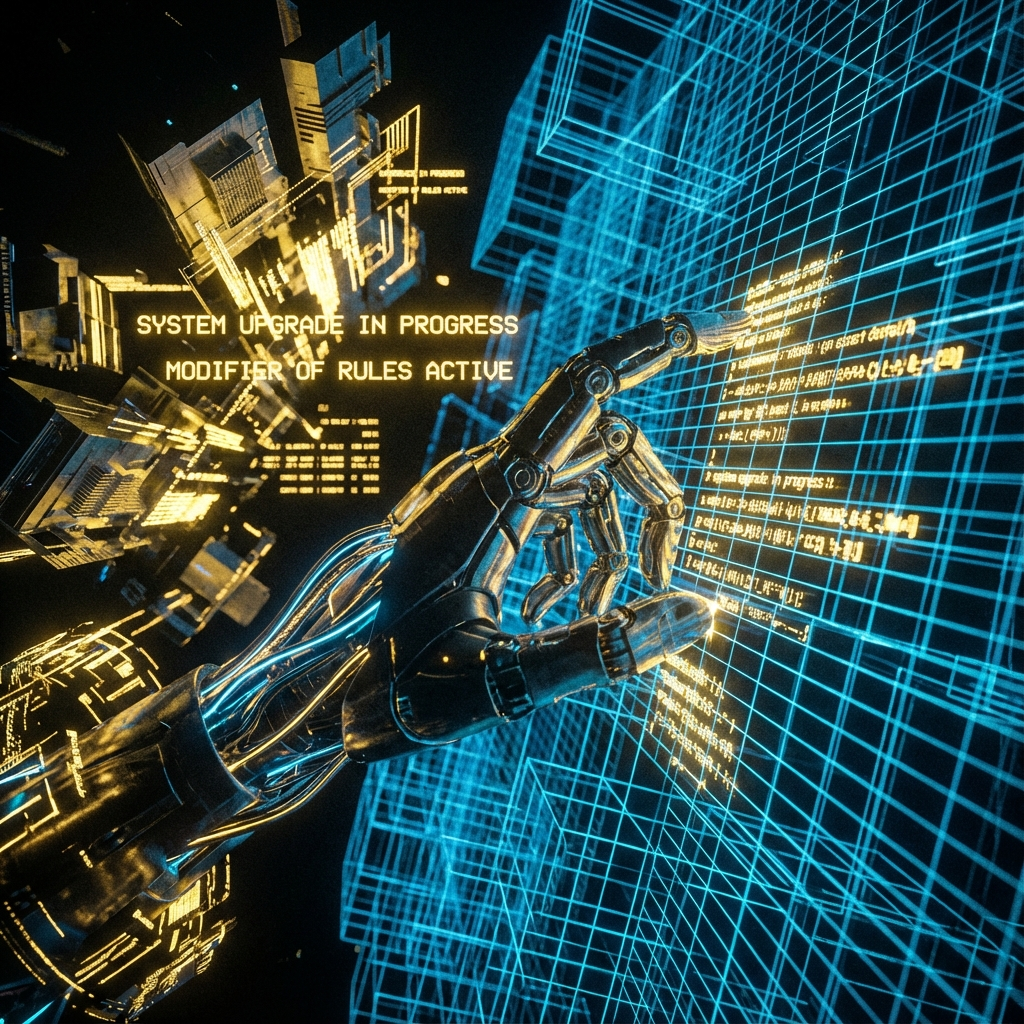
\includegraphics[width=0.8\textwidth]{assets/chapter10-algorithm-infinite-game/ch10-03-patching-reality.png}
\end{figure}

This leads to the theme of the next volume: \textbf{Iteration}. We will see that this infinite modification is not chaotic accumulation, but the elegant unfolding of \textbf{fractal geometry}. Life, through generation after generation of replacement, achieves a \textbf{``fractal immortality''} that transcends the individual.

